% !TEX TS-program = XeLaTeX
% Commands for running this example:
% 	 xelatex float-example
% 	 xelatex float-example
% End of Commands
\documentclass{book}
\pagestyle{empty}
\usepackage{tikz}
\usetikzlibrary{arrows}
\usepackage{bidituftefloat}
\let\plaintitle\relax % Why?
\let\plainauthor\relax % Why?
% Because bidituftefloat is a part of biditufte document classes and since \plainauthor and \plaintitle is undefined with the standard book class, we have to let it be \relax.
\usepackage[Kashida]{xepersian}
\begin{document}
بر خلاف اقتصاد خرد رفتارهای فردی شکل دهنده اقتصاد کلان نیست هر چند که از جمع رفتارهای فردی شکل گرفته‌است. کینز پدر علم اقتصاد نوین نمونه بارزی را از آثار رفتار واحدی را در عرصه کلان و خرد ارایه داده‌است که به تناقض پس‌انداز مشهور است. اگر افراد به صورت انفرادی پس انداز کنند در سالهای بعد دارای امکانات و قدرت مالی بیشتری خواهند بود و خواهند توانست که از سرمایه جمع شده خود استفاده کنند ولی اگر تمامی افراد جامعه هم‌زمان پس‌انداز خود را افزایش دهند و بخش بیشتری از درآمد خود را پس انداز نمایند مصرف کل اقتصاد پایین می‌آید و این امر موجب کاهش تولید نیز خواهد شد که این امر به کاهش درآمد افراد در آینده منجر می‌شود. از اینرو افزایش پس انداز برای اشخاص مفید می‌تواند باشد ولی برای جامعه به صورت کلی تأثیرات متفاوتی نسبت به تأثیرات فردی آن دارد.

\begin{figure}
\centering
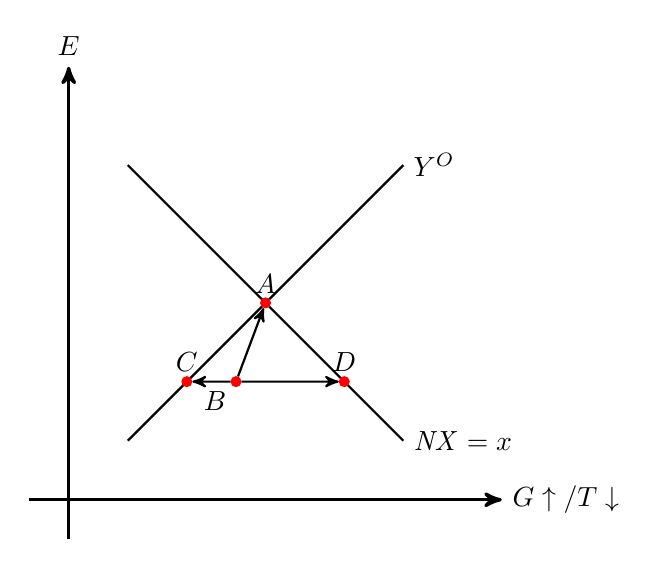
\begin{tikzpicture}[
    scale=5,
    axis/.style={very thick, ->, >=stealth'},
    important line/.style={thick},
    dashed line/.style={dashed, thin},
    pile/.style={thick, ->, >=stealth', shorten <=2pt, shorten
    >=2pt},
    every node/.style={color=black}
    ]
    % axis
    \draw[axis] (-0.1,0)  -- (1.1,0) node(xline)[right]
        {$G\uparrow/T\downarrow$};
    \draw[axis] (0,-0.1) -- (0,1.1) node(yline)[above] {$E$};
    % Lines
    \draw[important line] (.15,.15) coordinate (A) -- (.85,.85)
        coordinate (B) node[right, text width=5em] {$Y^O$};
    \draw[important line] (.15,.85) coordinate (C) -- (.85,.15)
        coordinate (D) node[right, text width=5em] {$\mathit{NX}=x$};
    % Intersection of lines
    \fill[red] (intersection cs:
       first line={(A) -- (B)},
       second line={(C) -- (D)}) coordinate (E) circle (.4pt)
       node[above,] {$A$};
    % The E point is placed more or less randomly
    \fill[red]  (E) +(-.075cm,-.2cm) coordinate (out) circle (.4pt)
        node[below left] {$B$};
    % Line connecting out and ext balances
    \draw [pile] (out) -- (intersection of A--B and out--[shift={(0:1pt)}]out)
        coordinate (extbal);
    \fill[red] (extbal) circle (.4pt) node[above] {$C$};
    % line connecting  out and int balances
    \draw [pile] (out) -- (intersection of C--D and out--[shift={(0:1pt)}]out)
        coordinate (intbal);
    \fill[red] (intbal) circle (.4pt) node[above] {$D$};
    % line between out og all balanced out :)
    \draw[pile] (out) -- (E);
\end{tikzpicture}
\caption{نمونه دیگر: اگر شرکتی یک یا چند تن از پرسنل خود را با ماشین‌آلات جایگزین نماید بی شک سود خواهد کرد و به نفع آن شرکت خواهد بود ولی اگر تمامی شرکتها به یکباره به این کار مبادرت ورزند بیکاری افزایش می‌یابد و موجب کاهش درآمد ملی و در نتیجه کاهش تقاضا برای تولیدات شرکتها شده و سود شرکتها را کاهش می‌دهد. از اینرو تأثیرات سطح کلان می‌تواند با تأثیرات در سطح خرد متضاد باشد.}
\end{figure}

بر خلاف اقتصاد خرد رفتارهای فردی شکل دهنده اقتصاد کلان نیست هر چند که از جمع رفتارهای فردی شکل گرفته‌است. کینز پدر علم اقتصاد نوین نمونه بارزی را از آثار رفتار واحدی را در عرصه کلان و خرد ارایه داده‌است که به تناقض پس‌انداز مشهور است. اگر افراد به صورت انفرادی پس انداز کنند در سالهای بعد دارای امکانات و قدرت مالی بیشتری خواهند بود و خواهند توانست که از سرمایه جمع شده خود استفاده کنند ولی اگر تمامی افراد جامعه هم‌زمان پس‌انداز خود را افزایش دهند و بخش بیشتری از درآمد خود را پس انداز نمایند مصرف کل اقتصاد پایین می‌آید و این امر موجب کاهش تولید نیز خواهد شد که این امر به کاهش درآمد افراد در آینده منجر می‌شود. از اینرو افزایش پس انداز برای اشخاص مفید می‌تواند باشد ولی برای جامعه به صورت کلی تأثیرات متفاوتی نسبت به تأثیرات فردی آن دارد.
\newpage
بر خلاف اقتصاد خرد رفتارهای فردی شکل دهنده اقتصاد کلان نیست هر چند که از جمع رفتارهای فردی شکل گرفته‌است. کینز پدر علم اقتصاد نوین نمونه بارزی را از آثار رفتار واحدی را در عرصه کلان و خرد ارایه داده‌است که به تناقض پس‌انداز مشهور است. اگر افراد به صورت انفرادی پس انداز کنند در سالهای بعد دارای امکانات و قدرت مالی بیشتری خواهند بود و خواهند توانست که از سرمایه جمع شده خود استفاده کنند ولی اگر تمامی افراد جامعه هم‌زمان پس‌انداز خود را افزایش دهند و بخش بیشتری از درآمد خود را پس انداز نمایند مصرف کل اقتصاد پایین می‌آید و این امر موجب کاهش تولید نیز خواهد شد که این امر به کاهش درآمد افراد در آینده منجر می‌شود. از اینرو افزایش پس انداز برای اشخاص مفید می‌تواند باشد ولی برای جامعه به صورت کلی تأثیرات متفاوتی نسبت به تأثیرات فردی آن دارد.

\begin{figure}
\centering
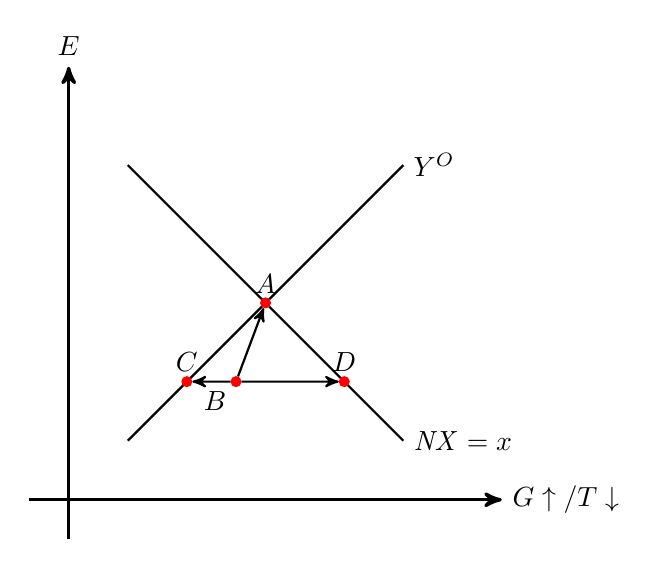
\begin{tikzpicture}[
    scale=5,
    axis/.style={very thick, ->, >=stealth'},
    important line/.style={thick},
    dashed line/.style={dashed, thin},
    pile/.style={thick, ->, >=stealth', shorten <=2pt, shorten
    >=2pt},
    every node/.style={color=black}
    ]
    % axis
    \draw[axis] (-0.1,0)  -- (1.1,0) node(xline)[right]
        {$G\uparrow/T\downarrow$};
    \draw[axis] (0,-0.1) -- (0,1.1) node(yline)[above] {$E$};
    % Lines
    \draw[important line] (.15,.15) coordinate (A) -- (.85,.85)
        coordinate (B) node[right, text width=5em] {$Y^O$};
    \draw[important line] (.15,.85) coordinate (C) -- (.85,.15)
        coordinate (D) node[right, text width=5em] {$\mathit{NX}=x$};
    % Intersection of lines
    \fill[red] (intersection cs:
       first line={(A) -- (B)},
       second line={(C) -- (D)}) coordinate (E) circle (.4pt)
       node[above,] {$A$};
    % The E point is placed more or less randomly
    \fill[red]  (E) +(-.075cm,-.2cm) coordinate (out) circle (.4pt)
        node[below left] {$B$};
    % Line connecting out and ext balances
    \draw [pile] (out) -- (intersection of A--B and out--[shift={(0:1pt)}]out)
        coordinate (extbal);
    \fill[red] (extbal) circle (.4pt) node[above] {$C$};
    % line connecting  out and int balances
    \draw [pile] (out) -- (intersection of C--D and out--[shift={(0:1pt)}]out)
        coordinate (intbal);
    \fill[red] (intbal) circle (.4pt) node[above] {$D$};
    % line between out og all balanced out :)
    \draw[pile] (out) -- (E);
\end{tikzpicture}
\caption{نمونه دیگر: اگر شرکتی یک یا چند تن از پرسنل خود را با ماشین‌آلات جایگزین نماید بی شک سود خواهد کرد و به نفع آن شرکت خواهد بود ولی اگر تمامی شرکتها به یکباره به این کار مبادرت ورزند بیکاری افزایش می‌یابد و موجب کاهش درآمد ملی و در نتیجه کاهش تقاضا برای تولیدات شرکتها شده و سود شرکتها را کاهش می‌دهد. از اینرو تأثیرات سطح کلان می‌تواند با تأثیرات در سطح خرد متضاد باشد.}
\end{figure}

بر خلاف اقتصاد خرد رفتارهای فردی شکل دهنده اقتصاد کلان نیست هر چند که از جمع رفتارهای فردی شکل گرفته‌است. کینز پدر علم اقتصاد نوین نمونه بارزی را از آثار رفتار واحدی را در عرصه کلان و خرد ارایه داده‌است که به تناقض پس‌انداز مشهور است. اگر افراد به صورت انفرادی پس انداز کنند در سالهای بعد دارای امکانات و قدرت مالی بیشتری خواهند بود و خواهند توانست که از سرمایه جمع شده خود استفاده کنند ولی اگر تمامی افراد جامعه هم‌زمان پس‌انداز خود را افزایش دهند و بخش بیشتری از درآمد خود را پس انداز نمایند مصرف کل اقتصاد پایین می‌آید و این امر موجب کاهش تولید نیز خواهد شد که این امر به کاهش درآمد افراد در آینده منجر می‌شود. از اینرو افزایش پس انداز برای اشخاص مفید می‌تواند باشد ولی برای جامعه به صورت کلی تأثیرات متفاوتی نسبت به تأثیرات فردی آن دارد.
\newpage
بر خلاف اقتصاد خرد رفتارهای فردی شکل دهنده اقتصاد کلان نیست هر چند که از جمع رفتارهای فردی شکل گرفته‌است. کینز پدر علم اقتصاد نوین نمونه بارزی را از آثار رفتار واحدی را در عرصه کلان و خرد ارایه داده‌است که به تناقض پس‌انداز مشهور است. اگر افراد به صورت انفرادی پس انداز کنند در سالهای بعد دارای امکانات و قدرت مالی بیشتری خواهند بود و خواهند توانست که از سرمایه جمع شده خود استفاده کنند ولی اگر تمامی افراد جامعه هم‌زمان پس‌انداز خود را افزایش دهند و بخش بیشتری از درآمد خود را پس انداز نمایند مصرف کل اقتصاد پایین می‌آید و این امر موجب کاهش تولید نیز خواهد شد که این امر به کاهش درآمد افراد در آینده منجر می‌شود. از اینرو افزایش پس انداز برای اشخاص مفید می‌تواند باشد ولی برای جامعه به صورت کلی تأثیرات متفاوتی نسبت به تأثیرات فردی آن دارد.

\begin{marginfigure}
\centering
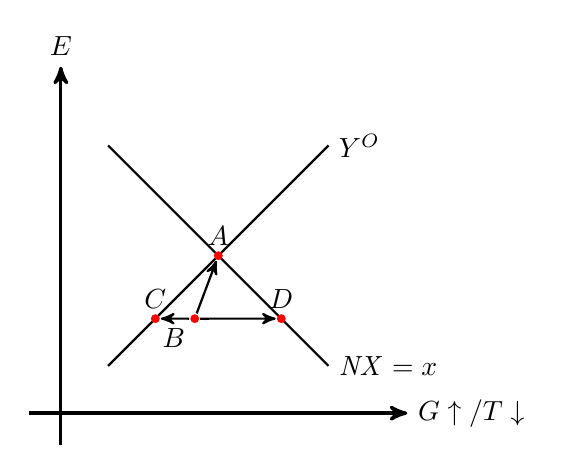
\begin{tikzpicture}[
    scale=4,
    axis/.style={very thick, ->, >=stealth'},
    important line/.style={thick},
    dashed line/.style={dashed, thin},
    pile/.style={thick, ->, >=stealth', shorten <=2pt, shorten
    >=2pt},
    every node/.style={color=black}
    ]
    % axis
    \draw[axis] (-0.1,0)  -- (1.1,0) node(xline)[right]
        {$G\uparrow/T\downarrow$};
    \draw[axis] (0,-0.1) -- (0,1.1) node(yline)[above] {$E$};
    % Lines
    \draw[important line] (.15,.15) coordinate (A) -- (.85,.85)
        coordinate (B) node[right, text width=5em] {$Y^O$};
    \draw[important line] (.15,.85) coordinate (C) -- (.85,.15)
        coordinate (D) node[right, text width=5em] {$\mathit{NX}=x$};
    % Intersection of lines
    \fill[red] (intersection cs:
       first line={(A) -- (B)},
       second line={(C) -- (D)}) coordinate (E) circle (.4pt)
       node[above,] {$A$};
    % The E point is placed more or less randomly
    \fill[red]  (E) +(-.075cm,-.2cm) coordinate (out) circle (.4pt)
        node[below left] {$B$};
    % Line connecting out and ext balances
    \draw [pile] (out) -- (intersection of A--B and out--[shift={(0:1pt)}]out)
        coordinate (extbal);
    \fill[red] (extbal) circle (.4pt) node[above] {$C$};
    % line connecting  out and int balances
    \draw [pile] (out) -- (intersection of C--D and out--[shift={(0:1pt)}]out)
        coordinate (intbal);
    \fill[red] (intbal) circle (.4pt) node[above] {$D$};
    % line between out og all balanced out :)
    \draw[pile] (out) -- (E);
\end{tikzpicture}
\caption{نمونه دیگر: اگر شرکتی یک یا چند تن از پرسنل خود را با ماشین‌آلات جایگزین نماید بی شک سود خواهد کرد و به نفع آن شرکت خواهد بود ولی اگر تمامی شرکتها به یکباره به این کار مبادرت ورزند بیکاری افزایش می‌یابد و موجب کاهش درآمد ملی و در نتیجه کاهش تقاضا برای تولیدات شرکتها شده و سود شرکتها را کاهش می‌دهد. از اینرو تأثیرات سطح کلان می‌تواند با تأثیرات در سطح خرد متضاد باشد.}
\end{marginfigure}

بر خلاف اقتصاد خرد رفتارهای فردی شکل دهنده اقتصاد کلان نیست هر چند که از جمع رفتارهای فردی شکل گرفته‌است. کینز پدر علم اقتصاد نوین نمونه بارزی را از آثار رفتار واحدی را در عرصه کلان و خرد ارایه داده‌است که به تناقض پس‌انداز مشهور است. اگر افراد به صورت انفرادی پس انداز کنند در سالهای بعد دارای امکانات و قدرت مالی بیشتری خواهند بود و خواهند توانست که از سرمایه جمع شده خود استفاده کنند ولی اگر تمامی افراد جامعه هم‌زمان پس‌انداز خود را افزایش دهند و بخش بیشتری از درآمد خود را پس انداز نمایند مصرف کل اقتصاد پایین می‌آید و این امر موجب کاهش تولید نیز خواهد شد که این امر به کاهش درآمد افراد در آینده منجر می‌شود. از اینرو افزایش پس انداز برای اشخاص مفید می‌تواند باشد ولی برای جامعه به صورت کلی تأثیرات متفاوتی نسبت به تأثیرات فردی آن دارد.
\newpage
بر خلاف اقتصاد خرد رفتارهای فردی شکل دهنده اقتصاد کلان نیست هر چند که از جمع رفتارهای فردی شکل گرفته‌است. کینز پدر علم اقتصاد نوین نمونه بارزی را از آثار رفتار واحدی را در عرصه کلان و خرد ارایه داده‌است که به تناقض پس‌انداز مشهور است. اگر افراد به صورت انفرادی پس انداز کنند در سالهای بعد دارای امکانات و قدرت مالی بیشتری خواهند بود و خواهند توانست که از سرمایه جمع شده خود استفاده کنند ولی اگر تمامی افراد جامعه هم‌زمان پس‌انداز خود را افزایش دهند و بخش بیشتری از درآمد خود را پس انداز نمایند مصرف کل اقتصاد پایین می‌آید و این امر موجب کاهش تولید نیز خواهد شد که این امر به کاهش درآمد افراد در آینده منجر می‌شود. از اینرو افزایش پس انداز برای اشخاص مفید می‌تواند باشد ولی برای جامعه به صورت کلی تأثیرات متفاوتی نسبت به تأثیرات فردی آن دارد.

\begin{marginfigure}
\centering
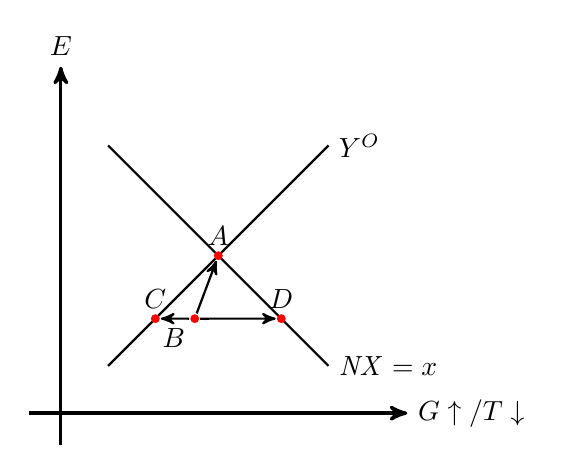
\begin{tikzpicture}[
    scale=4,
    axis/.style={very thick, ->, >=stealth'},
    important line/.style={thick},
    dashed line/.style={dashed, thin},
    pile/.style={thick, ->, >=stealth', shorten <=2pt, shorten
    >=2pt},
    every node/.style={color=black}
    ]
    % axis
    \draw[axis] (-0.1,0)  -- (1.1,0) node(xline)[right]
        {$G\uparrow/T\downarrow$};
    \draw[axis] (0,-0.1) -- (0,1.1) node(yline)[above] {$E$};
    % Lines
    \draw[important line] (.15,.15) coordinate (A) -- (.85,.85)
        coordinate (B) node[right, text width=5em] {$Y^O$};
    \draw[important line] (.15,.85) coordinate (C) -- (.85,.15)
        coordinate (D) node[right, text width=5em] {$\mathit{NX}=x$};
    % Intersection of lines
    \fill[red] (intersection cs:
       first line={(A) -- (B)},
       second line={(C) -- (D)}) coordinate (E) circle (.4pt)
       node[above,] {$A$};
    % The E point is placed more or less randomly
    \fill[red]  (E) +(-.075cm,-.2cm) coordinate (out) circle (.4pt)
        node[below left] {$B$};
    % Line connecting out and ext balances
    \draw [pile] (out) -- (intersection of A--B and out--[shift={(0:1pt)}]out)
        coordinate (extbal);
    \fill[red] (extbal) circle (.4pt) node[above] {$C$};
    % line connecting  out and int balances
    \draw [pile] (out) -- (intersection of C--D and out--[shift={(0:1pt)}]out)
        coordinate (intbal);
    \fill[red] (intbal) circle (.4pt) node[above] {$D$};
    % line between out og all balanced out :)
    \draw[pile] (out) -- (E);
\end{tikzpicture}
\caption{نمونه دیگر: اگر شرکتی یک یا چند تن از پرسنل خود را با ماشین‌آلات جایگزین نماید بی شک سود خواهد کرد و به نفع آن شرکت خواهد بود ولی اگر تمامی شرکتها به یکباره به این کار مبادرت ورزند بیکاری افزایش می‌یابد و موجب کاهش درآمد ملی و در نتیجه کاهش تقاضا برای تولیدات شرکتها شده و سود شرکتها را کاهش می‌دهد. از اینرو تأثیرات سطح کلان می‌تواند با تأثیرات در سطح خرد متضاد باشد.}
\end{marginfigure}

بر خلاف اقتصاد خرد رفتارهای فردی شکل دهنده اقتصاد کلان نیست هر چند که از جمع رفتارهای فردی شکل گرفته‌است. کینز پدر علم اقتصاد نوین نمونه بارزی را از آثار رفتار واحدی را در عرصه کلان و خرد ارایه داده‌است که به تناقض پس‌انداز مشهور است. اگر افراد به صورت انفرادی پس انداز کنند در سالهای بعد دارای امکانات و قدرت مالی بیشتری خواهند بود و خواهند توانست که از سرمایه جمع شده خود استفاده کنند ولی اگر تمامی افراد جامعه هم‌زمان پس‌انداز خود را افزایش دهند و بخش بیشتری از درآمد خود را پس انداز نمایند مصرف کل اقتصاد پایین می‌آید و این امر موجب کاهش تولید نیز خواهد شد که این امر به کاهش درآمد افراد در آینده منجر می‌شود. از اینرو افزایش پس انداز برای اشخاص مفید می‌تواند باشد ولی برای جامعه به صورت کلی تأثیرات متفاوتی نسبت به تأثیرات فردی آن دارد.
\newpage
بر خلاف اقتصاد خرد رفتارهای فردی شکل دهنده اقتصاد کلان نیست هر چند که از جمع رفتارهای فردی شکل گرفته‌است. کینز پدر علم اقتصاد نوین نمونه بارزی را از آثار رفتار واحدی را در عرصه کلان و خرد ارایه داده‌است که به تناقض پس‌انداز مشهور است. اگر افراد به صورت انفرادی پس انداز کنند در سالهای بعد دارای امکانات و قدرت مالی بیشتری خواهند بود و خواهند توانست که از سرمایه جمع شده خود استفاده کنند ولی اگر تمامی افراد جامعه هم‌زمان پس‌انداز خود را افزایش دهند و بخش بیشتری از درآمد خود را پس انداز نمایند مصرف کل اقتصاد پایین می‌آید و این امر موجب کاهش تولید نیز خواهد شد که این امر به کاهش درآمد افراد در آینده منجر می‌شود. از اینرو افزایش پس انداز برای اشخاص مفید می‌تواند باشد ولی برای جامعه به صورت کلی تأثیرات متفاوتی نسبت به تأثیرات فردی آن دارد.

\begin{figure*}
\centering
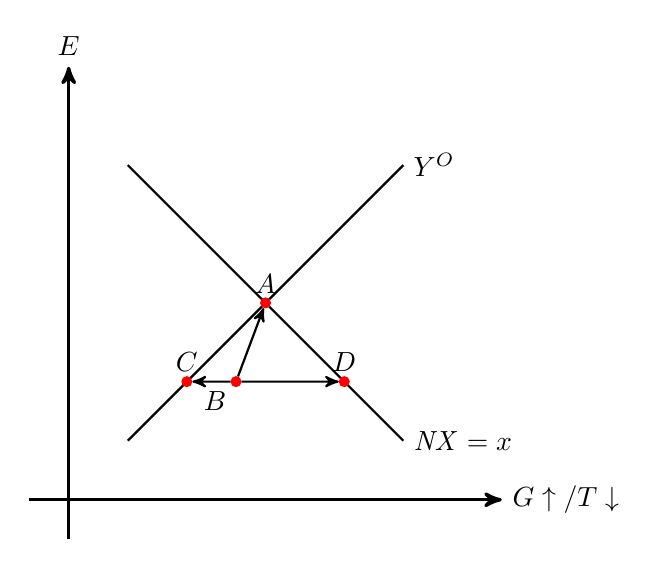
\begin{tikzpicture}[
    scale=5,
    axis/.style={very thick, ->, >=stealth'},
    important line/.style={thick},
    dashed line/.style={dashed, thin},
    pile/.style={thick, ->, >=stealth', shorten <=2pt, shorten
    >=2pt},
    every node/.style={color=black}
    ]
    % axis
    \draw[axis] (-0.1,0)  -- (1.1,0) node(xline)[right]
        {$G\uparrow/T\downarrow$};
    \draw[axis] (0,-0.1) -- (0,1.1) node(yline)[above] {$E$};
    % Lines
    \draw[important line] (.15,.15) coordinate (A) -- (.85,.85)
        coordinate (B) node[right, text width=5em] {$Y^O$};
    \draw[important line] (.15,.85) coordinate (C) -- (.85,.15)
        coordinate (D) node[right, text width=5em] {$\mathit{NX}=x$};
    % Intersection of lines
    \fill[red] (intersection cs:
       first line={(A) -- (B)},
       second line={(C) -- (D)}) coordinate (E) circle (.4pt)
       node[above,] {$A$};
    % The E point is placed more or less randomly
    \fill[red]  (E) +(-.075cm,-.2cm) coordinate (out) circle (.4pt)
        node[below left] {$B$};
    % Line connecting out and ext balances
    \draw [pile] (out) -- (intersection of A--B and out--[shift={(0:1pt)}]out)
        coordinate (extbal);
    \fill[red] (extbal) circle (.4pt) node[above] {$C$};
    % line connecting  out and int balances
    \draw [pile] (out) -- (intersection of C--D and out--[shift={(0:1pt)}]out)
        coordinate (intbal);
    \fill[red] (intbal) circle (.4pt) node[above] {$D$};
    % line between out og all balanced out :)
    \draw[pile] (out) -- (E);
\end{tikzpicture}
\caption{نمونه دیگر: اگر شرکتی یک یا چند تن از پرسنل خود را با ماشین‌آلات جایگزین نماید بی شک سود خواهد کرد و به نفع آن شرکت خواهد بود ولی اگر تمامی شرکتها به یکباره به این کار مبادرت ورزند بیکاری افزایش می‌یابد و موجب کاهش درآمد ملی و در نتیجه کاهش تقاضا برای تولیدات شرکتها شده و سود شرکتها را کاهش می‌دهد. از اینرو تأثیرات سطح کلان می‌تواند با تأثیرات در سطح خرد متضاد باشد.}
\end{figure*}

بر خلاف اقتصاد خرد رفتارهای فردی شکل دهنده اقتصاد کلان نیست هر چند که از جمع رفتارهای فردی شکل گرفته‌است. کینز پدر علم اقتصاد نوین نمونه بارزی را از آثار رفتار واحدی را در عرصه کلان و خرد ارایه داده‌است که به تناقض پس‌انداز مشهور است. اگر افراد به صورت انفرادی پس انداز کنند در سالهای بعد دارای امکانات و قدرت مالی بیشتری خواهند بود و خواهند توانست که از سرمایه جمع شده خود استفاده کنند ولی اگر تمامی افراد جامعه هم‌زمان پس‌انداز خود را افزایش دهند و بخش بیشتری از درآمد خود را پس انداز نمایند مصرف کل اقتصاد پایین می‌آید و این امر موجب کاهش تولید نیز خواهد شد که این امر به کاهش درآمد افراد در آینده منجر می‌شود. از اینرو افزایش پس انداز برای اشخاص مفید می‌تواند باشد ولی برای جامعه به صورت کلی تأثیرات متفاوتی نسبت به تأثیرات فردی آن دارد.
\newpage
بر خلاف اقتصاد خرد رفتارهای فردی شکل دهنده اقتصاد کلان نیست هر چند که از جمع رفتارهای فردی شکل گرفته‌است. کینز پدر علم اقتصاد نوین نمونه بارزی را از آثار رفتار واحدی را در عرصه کلان و خرد ارایه داده‌است که به تناقض پس‌انداز مشهور است. اگر افراد به صورت انفرادی پس انداز کنند در سالهای بعد دارای امکانات و قدرت مالی بیشتری خواهند بود و خواهند توانست که از سرمایه جمع شده خود استفاده کنند ولی اگر تمامی افراد جامعه هم‌زمان پس‌انداز خود را افزایش دهند و بخش بیشتری از درآمد خود را پس انداز نمایند مصرف کل اقتصاد پایین می‌آید و این امر موجب کاهش تولید نیز خواهد شد که این امر به کاهش درآمد افراد در آینده منجر می‌شود. از اینرو افزایش پس انداز برای اشخاص مفید می‌تواند باشد ولی برای جامعه به صورت کلی تأثیرات متفاوتی نسبت به تأثیرات فردی آن دارد.

\begin{figure*}
\centering
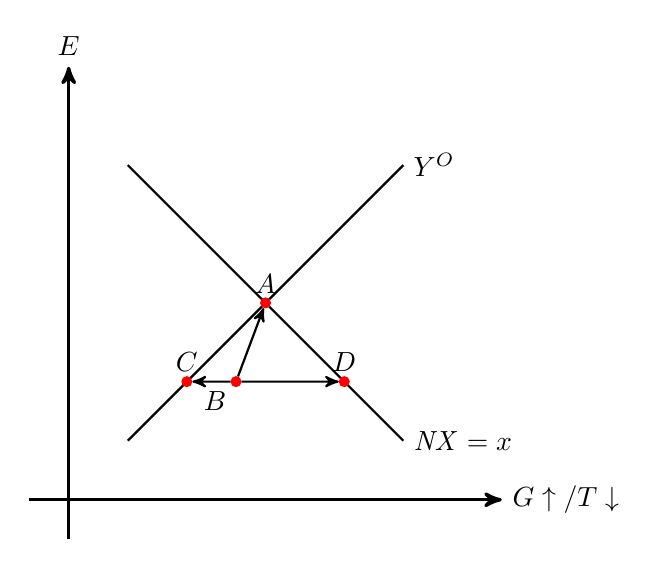
\begin{tikzpicture}[
    scale=5,
    axis/.style={very thick, ->, >=stealth'},
    important line/.style={thick},
    dashed line/.style={dashed, thin},
    pile/.style={thick, ->, >=stealth', shorten <=2pt, shorten
    >=2pt},
    every node/.style={color=black}
    ]
    % axis
    \draw[axis] (-0.1,0)  -- (1.1,0) node(xline)[right]
        {$G\uparrow/T\downarrow$};
    \draw[axis] (0,-0.1) -- (0,1.1) node(yline)[above] {$E$};
    % Lines
    \draw[important line] (.15,.15) coordinate (A) -- (.85,.85)
        coordinate (B) node[right, text width=5em] {$Y^O$};
    \draw[important line] (.15,.85) coordinate (C) -- (.85,.15)
        coordinate (D) node[right, text width=5em] {$\mathit{NX}=x$};
    % Intersection of lines
    \fill[red] (intersection cs:
       first line={(A) -- (B)},
       second line={(C) -- (D)}) coordinate (E) circle (.4pt)
       node[above,] {$A$};
    % The E point is placed more or less randomly
    \fill[red]  (E) +(-.075cm,-.2cm) coordinate (out) circle (.4pt)
        node[below left] {$B$};
    % Line connecting out and ext balances
    \draw [pile] (out) -- (intersection of A--B and out--[shift={(0:1pt)}]out)
        coordinate (extbal);
    \fill[red] (extbal) circle (.4pt) node[above] {$C$};
    % line connecting  out and int balances
    \draw [pile] (out) -- (intersection of C--D and out--[shift={(0:1pt)}]out)
        coordinate (intbal);
    \fill[red] (intbal) circle (.4pt) node[above] {$D$};
    % line between out og all balanced out :)
    \draw[pile] (out) -- (E);
\end{tikzpicture}
\caption{نمونه دیگر: اگر شرکتی یک یا چند تن از پرسنل خود را با ماشین‌آلات جایگزین نماید بی شک سود خواهد کرد و به نفع آن شرکت خواهد بود ولی اگر تمامی شرکتها به یکباره به این کار مبادرت ورزند بیکاری افزایش می‌یابد و موجب کاهش درآمد ملی و در نتیجه کاهش تقاضا برای تولیدات شرکتها شده و سود شرکتها را کاهش می‌دهد. از اینرو تأثیرات سطح کلان می‌تواند با تأثیرات در سطح خرد متضاد باشد.}
\end{figure*}

بر خلاف اقتصاد خرد رفتارهای فردی شکل دهنده اقتصاد کلان نیست هر چند که از جمع رفتارهای فردی شکل گرفته‌است. کینز پدر علم اقتصاد نوین نمونه بارزی را از آثار رفتار واحدی را در عرصه کلان و خرد ارایه داده‌است که به تناقض پس‌انداز مشهور است. اگر افراد به صورت انفرادی پس انداز کنند در سالهای بعد دارای امکانات و قدرت مالی بیشتری خواهند بود و خواهند توانست که از سرمایه جمع شده خود استفاده کنند ولی اگر تمامی افراد جامعه هم‌زمان پس‌انداز خود را افزایش دهند و بخش بیشتری از درآمد خود را پس انداز نمایند مصرف کل اقتصاد پایین می‌آید و این امر موجب کاهش تولید نیز خواهد شد که این امر به کاهش درآمد افراد در آینده منجر می‌شود. از اینرو افزایش پس انداز برای اشخاص مفید می‌تواند باشد ولی برای جامعه به صورت کلی تأثیرات متفاوتی نسبت به تأثیرات فردی آن دارد.
\end{document}